\documentclass{handout}

% \SetInstructor{ Lt Col James Phillips}
\SetCourseTitle{ECE231: Electrical Circuits and Systems I}
\SetSemester{Fall 2016}
\SetHandoutTitle{Lecture 1: Introduction \& Signal Variables}
%\SetDueDate{1 Jan 2016}
%\ShowAllBlanks



\showsoln \setsolncolor{red}

\begin{document}
\maketitle

\textbf{OBJECTIVES:}
\begin{enumerate}
\item Introduce yourselves
\item Review syllabus and course website
\item Review engineering notation
\item Introduce basic electrical variables
\item Introduce Passive Sign Convention
\end{enumerate}

\textbf{READING}
\begin{description}
\item [Required]:
\begin{itemize}
\item  Textbook, sections 1.1--1.3, pages 1--10
\item Course website \em{\textbf{https://sharepoint.usafa.edu/academics/eleccompengineering/ece231/default.aspx}}\em
\end{itemize}
\item [Optional]: {\em https://learn.sparkfun.com/tutorials/voltage-current-resistance-and-ohms-law}
\end{description}



\section{Engineering Notation}

What is engineering notation \& why do we use it?
\soln{3in}{
\begin{itemize}
\item A way or representing very large or very small numbers
\item Uses a coefficient multiplied by a power of 10
\item Exponents are ALWAYS  a power of 3
\end{itemize}
}

See Table \ref{tab: Eng Prefixes} for common engineering prefixes and their values.

\begin{table}[h]
\centering
\begin{tabular}{|l|c|c|}
\hline
Prefix & Abbreviation & Value \\
\hline \hline
Giga & $G$ & $10^9$ \\
Mega & $M$ & $10^6$ \\
Kilo & $k$ & $10^3$ \\
\hline
milli & $m$ & $10^{-3}$ \\
micro & $\mu$ & $10^{-6}$ \\
nano & $n$ & $10^{-9}$ \\
pico & $p$ & $10^{-12}$ \\
\hline
\end{tabular}
\caption{Engineering prefixes and values}
\label{tab: Eng Prefixes}
\end{table}


\em {\large{\textbf{Example: Convert the following to engineering notation}}} \em
\vspace{10pt}
\\
\vspace{10pt}
$3.014 \times 10^7 \ V$ \\
\vspace{10pt}
$0.00003056\ W$ \\
\vspace{10pt}
$2,586,720\ \Omega$

\begin{center}
\soln{2.5in}{
$3.014 \times 10^7\  V \rightarrow 30.14 \times 10^6\  V \rightarrow 30.14\  MV$ \\
\vspace{10pt}
$0.00003056\  W \rightarrow 30.56 \times 10^{-6}\  W \rightarrow 30.56 {\mu}\ W$ \\
\vspace{10pt}
$2,586,720\  \Omega \rightarrow 2.586 \times 10^6 \  \Omega \rightarrow 2.586 \ M\Omega$
}
\end{center}

\section{Electrical Variables}
The most basic quantities in Electrical Engineering are Charge ($q$) measured in coulombs ($C$) and Energy ($w$) measured in Joules ($J$).  You should have a reasonable understanding of these quantities from Physics.  We will build on these basics to develop the concept of current, voltage and power.

\subsection{Current}
Current is the defined as the change in charge over time and is {\em measured through a single point (or small area like a wire cross section)}. Current is mathematically defined as:

\soln{1in}{
\begin{equation}
i=\frac{\partial q}{\partial t}
\end{equation}
}

The SI unit for current is the ampere or amp which is defined as $1\ A = \frac{1\ coulomb}{1\ second}$. Even though current is caused by the flow of electrons, we define current to be in the direction of positive charge movement.  ELECTRONS FLOW IN THE OPPISITE DIRECTION AS OUR MEASURED CURRENT!

\subsection{Voltage}
Next we need to define voltage.  Voltage is the change in energy experienced by a charge moving in a circuit. {\em Voltage is measured between 2 points and is independent of the path taken through the circuit. }
If a charge ($q$) moved from $A$ to $B$ in a circuit and experienced a change in energy of $\partial w$ then there is a voltage between $A$ and $B$ defined by:
\soln{1in}{
\begin{equation}
v = \frac{\partial w}{\partial q}
\end{equation}
}

The SI unit for voltage is the volt which is defines as $1\ V = \frac{1\ Joule}{1\ coulomb}$.

An alternate definition for voltage is:
\soln{1in}{
\begin{equation}
v = \frac{\partial \lambda}{\partial t}
\end{equation}
}

where $\lambda$ is magnetic flux.  We will not rely on this definition (at least for now).

\subsection{Power}
Voltage and current are not very useful unless we can use them to do work, and to do work requires power!  Power the change in energy per unit time and is in general defined by:
\soln{1in}{
\begin{equation}
P = \frac{\partial w}{\partial t}
\end{equation}
}

The SI unit for power is watts ($W$) where $1\ Watt = \frac{1\ Joule}{1\ second}$. {\em Power is measured in (or at) a circuit element!}

\subsection{Resistance}
Electricity will not flow in a circuit unimpeded, therefore, we need to define the concept of resistance.  Resistance is simply the degree to which the flow of current is opposed in a circuit element.  A circuit element with a larger resistance will have a smaller current though it than a smaller resistance (if all other variables are constant).  The SI unit for resistance is the Ohm ($\Omega$).  $1 \ \Omega = \frac{1\ volt}{1\ amp}$.

\newpage
\pagebreak
\clearpage

\section{Passive Sign Convention}
Before we move on to Ohm's Law and the Power lay we must learn a ''rule of thumb'' for how we assign currents and voltages in a circuit.  The rule of thumb is called the passive sign convention (PSC) and is shown in Figure \ref{fig: PSC}.  Notice for every device in the diagram, we have assigned the current entering the positive (voltage) terminal.

\begin{figure}[h t b]
\centering
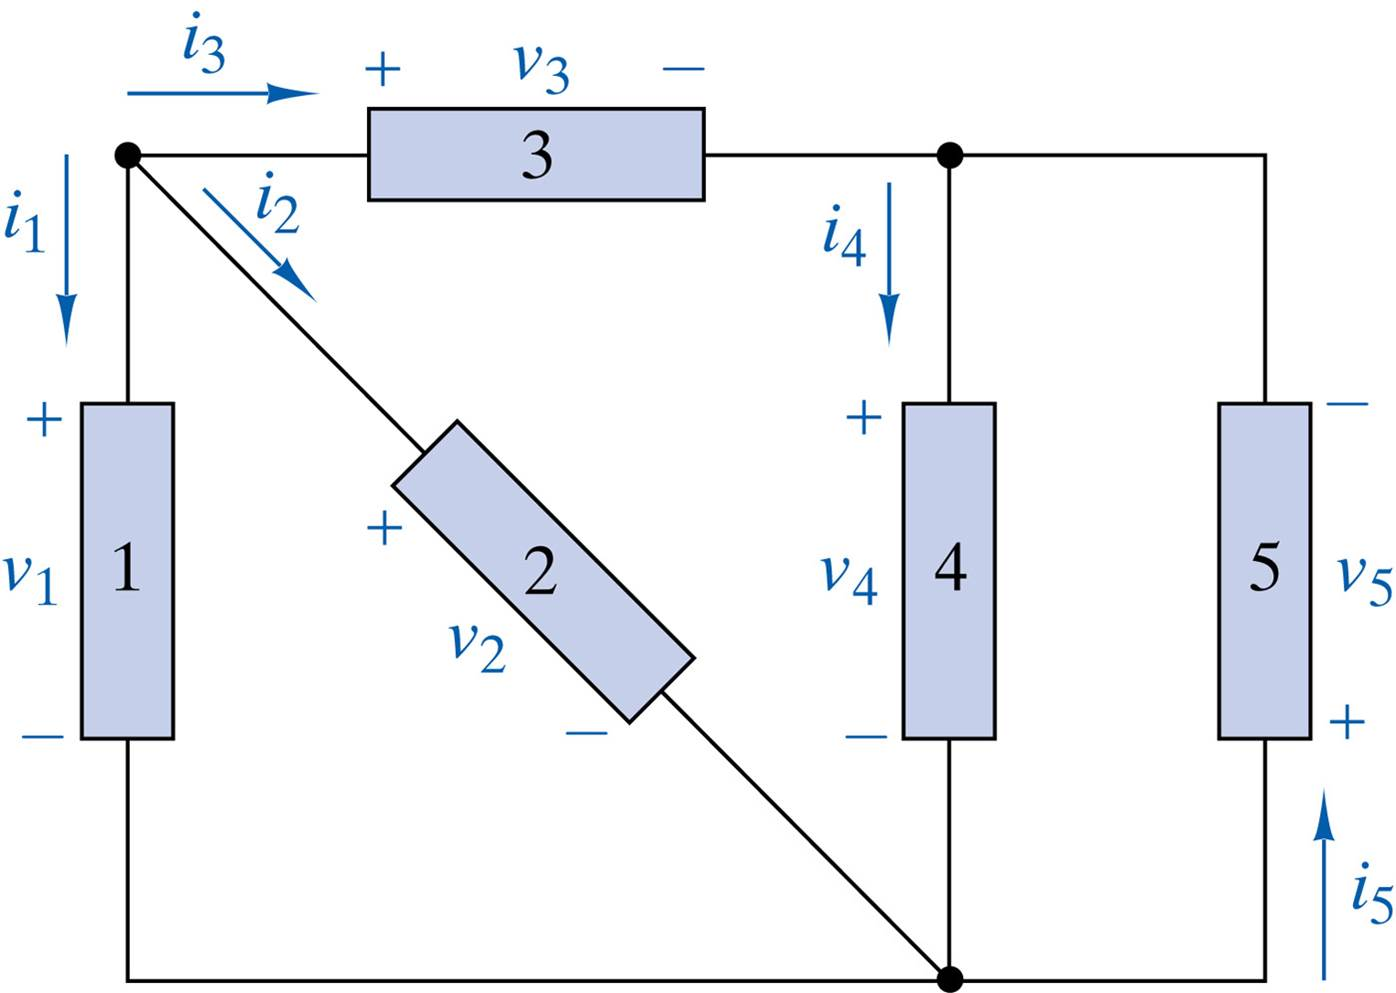
\includegraphics[width=0.5\textwidth]{Passive_Sign_Convention.jpg}
\caption{A basic circuit showing the passive sign convention}
\label{fig: PSC}
\end{figure}

Steps for applying the PSC:
\soln{3in}{
\begin{enumerate}
\item Assign voltage polarities across all circuit elements.  Use your best guess as to which direction the voltage should be assigned.  If your guess is wrong, do not worry; the math will fix it for you.
\item Assign current directions into the positive voltage terminal of each device
\end{enumerate}
}

In this class, it will be of great benefit to learn to consistently apply the PSC!

\section{Ohm's Law and the Power Law}

Now we will move into defining how Voltage, Current, Power and Resistance are all related.

\subsection{Ohm's law}
We have already talked about the concept of resistance, but we need to introduce a new device called a resistor.  A resistor is a linear circuit element that has resistance.  When we refer to a {\em linear device} we are saying that its current voltage relationsip is a straight line that passes through the origin.  Also the slope is the measure of device's resistance.  This leads us to Ohm's Law:

\soln{1.5in}{
\begin{equation} \label{eq:Ohms_law}
v = iR
\end{equation}
}

This relationship is shown graphically in Figure \ref{fig: Ohms_law}.  Notice in the figure that the PSC has been properly applied.

\begin{figure}
\centering
\soln{2in}{
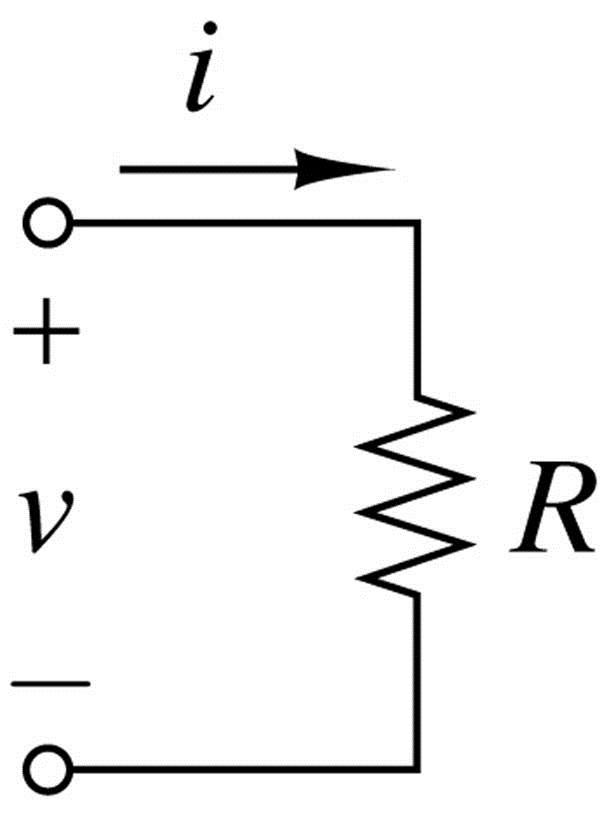
\includegraphics[width=0.25\textwidth]{Ohms_law.jpg}
}
\caption{Ohm's Law in pictures.....}
\label{fig: Ohms_law}
\end{figure}

\textbf{Example:}  Figure \ref{fig: OhmsLawExample} shows a simple circuit made up of an ideal voltage source and a resistor.  Assign a voltage polarity and a current direction based on the passive sign convention; then find the current.

\begin{figure}
\centering
\soln{2in}{
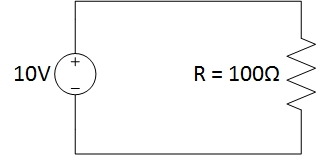
\includegraphics[width=0.5\textwidth]{OhmsLawExample.jpg}
}
\caption{Ohm's Law example circuit}
\label{fig: OhmsLawExample}
\end{figure}

\soln{4in}{Figure \ref{fig: OhmsLawExampleSolution} shows the voltage polarity and current directions.

\begin{eqnarray}
i_R &=&\frac{v_R}{R} \nonumber\\
i_R &=&\frac{10\ V}{100}\ \Omega \\
i_R &=& 100\ mA \nonumber
\end{eqnarray}

I hope it is obvious that $v_R = 10\ V$ but if not it will be in a few lessons.  Since $i_R = 100\ mA$,$ i_S = -100\ mA$.

}

\begin{figure}
\centering
\soln{2in}{
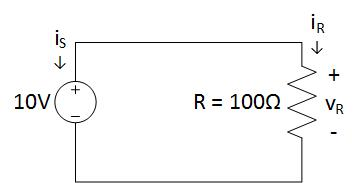
\includegraphics[width=0.5\textwidth]{OhmsLawExampleSolution.jpg}
}
\caption{Ohm's Law example circuit}
\label{fig: OhmsLawExampleSolution}
\end{figure}


\subsection{Power Law}
We just defined a relationship between voltage ($v$), current ($i$) and resistance ($R$); but we are ultimately interested in producing and utilizing power.  We want to get work done!  How do $v$, $i$, and $R$, relate to power ($P$)?

Recall that $P = \frac{\partial w}{\partial t}$,  $v = \frac{\partial w}{\partial q}$, and $i = \frac{\partial q}{\partial t}$; therefore since:

\begin{equation}
 \frac{\partial w}{\partial t} =  \frac{\partial w}{\partial q} \frac{\partial q}{\partial t}
\end{equation}

then

\soln{1.5in}{
\begin{equation}
P=vi
\end{equation}
}

If we apply this equation to devices in a circuit where the PSC was used:

\soln{2in}{

\begin{description}
\item [$\mathbf{P>0}$] means a device is consuming power
\item [$\mathbf{P<0}$] means a device is providing power
\end{description}
}

Using Ohm's Law we can develop alternative versions of the Power Law:

\soln{1.5in}{
\begin{equation}
P=i^2R
\end{equation}
}

\soln{1.5in}{
\begin{equation}
P=\frac{v^2}{R}
\end{equation}
}

\textbf{Example:} Let's revisit Figure \ref{fig: OhmsLawExample} and find the power at the source and the resistor.  Also, show that the resistor consumes power while the source provides power.


\soln{6in}{
Recall:
\begin{eqnarray}
v_S &=& 10\ V \nonumber \\
i_S &=& -100\ mA \nonumber \\
v_R &=& 10\ V  \\
i_R &=& 100\ mA \nonumber \\
R &=& 100\ \Omega \nonumber
\end{eqnarray}

Source power is simply
\begin{eqnarray}
P_S &=& v_Si_S \nonumber \\
P_S &=& 10\ V \times (-100\ mA) \\
P_S &=& -1\ W  \nonumber
\end{eqnarray}
Notice, since the power is negative, by the PSC the source provides power!

For the resistor power we can use any of our power equations, but lets use $P=i^2R$.

\begin
{eqnarray}
P_R &=& i_R^2R \nonumber \\
P_R &=& (100\ mA)^2 \times 100\ \Omega \nonumber \\
P_R &=& (100 \times 10^{-3}\ A)^2 \times 100\ \Omega \\
P_R &=& 10000 \times 10^{-6}\ A^2  \times 100\ \Omega \nonumber \\
P_R &=& 1\ W  \nonumber
\end{eqnarray}

Notice in this example, I worked out all the math long hand and carried my units through to the answer.  If you are interested enough you can check the diminsional analysis and verify that $A^2 \times \Omega$ is indeed $Watts$.

}


\section{Review Questions}
\begin{questions}
\item What unit is used to measure current?

\soln{1in}{Amperes or Amps}

\item Does conservation of power hold in electrical circuits?

\soln{1in}{Yes}

\newpage


\end{questions}

\end{document}
